\section{Passive Decomposition}

\begin{frame}
	\frametitle{Passive Decomposition}
	
	\begin{itemize}
		\item First introduced by D. Lee 2008. \footcite{LeePassive}
		\item Proposed system dynamics split:
		\begin{itemize}
			\item Shape	- internal configuration of each robot
			\item Locked - current overall behavior of multiple robot systems 
			\item Coupled - interaction between locked and shape dynamics
		\end{itemize}
		\item Passive decomposition
		\begin{itemize}
			\item Applying a control law to cancel the dynamics coupling terms without energy generation
			\item Enforces energetic passivity
		\end{itemize}
	\end{itemize}
\end{frame}

\begin{frame}
	\frametitle{Passive Decomposition - Application \footcite{passive-decomp-quadrotor-with-robotic-manip}        \footcite{decoupled-aerial-manipulation}}
	
	\begin{columns}
		\begin{column}{0.5\textwidth}\centering
			\begin{figure}[H]
				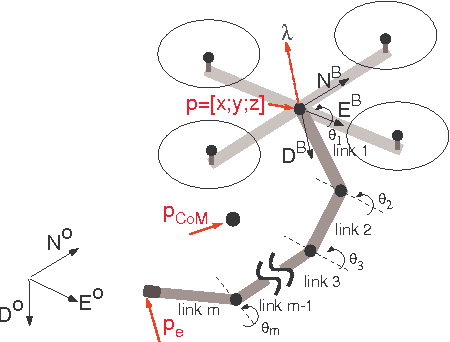
\includegraphics[width=\columnwidth]{figures/aerial_manip.png}	
				\centering
				\label{fig:aerial_manip}
			\end{figure}
		\end{column}
		
		\begin{column}{0.5\textwidth}\centering
			\begin{itemize}
			\item Quadrotor-manipulator system dynamics can be completely decoupled into:
			\begin{itemize}
				\item the center-of-mass dynamics in E(3)
				\item Lagrange dynamics of robotic manipulator with full-actuation and no gravity effect
			\end{itemize}
			\end{itemize}
		\end{column}
	\end{columns}
 \end{frame}

\begin{frame}
	\frametitle{Passive Decomposition - Payload Transportation}
\end{frame}